% !TeX root = ../main.tex
\begin{frame}
    \frametitle{How we got here}
    \centering
    \wait
    \raisebox{-3em}{
        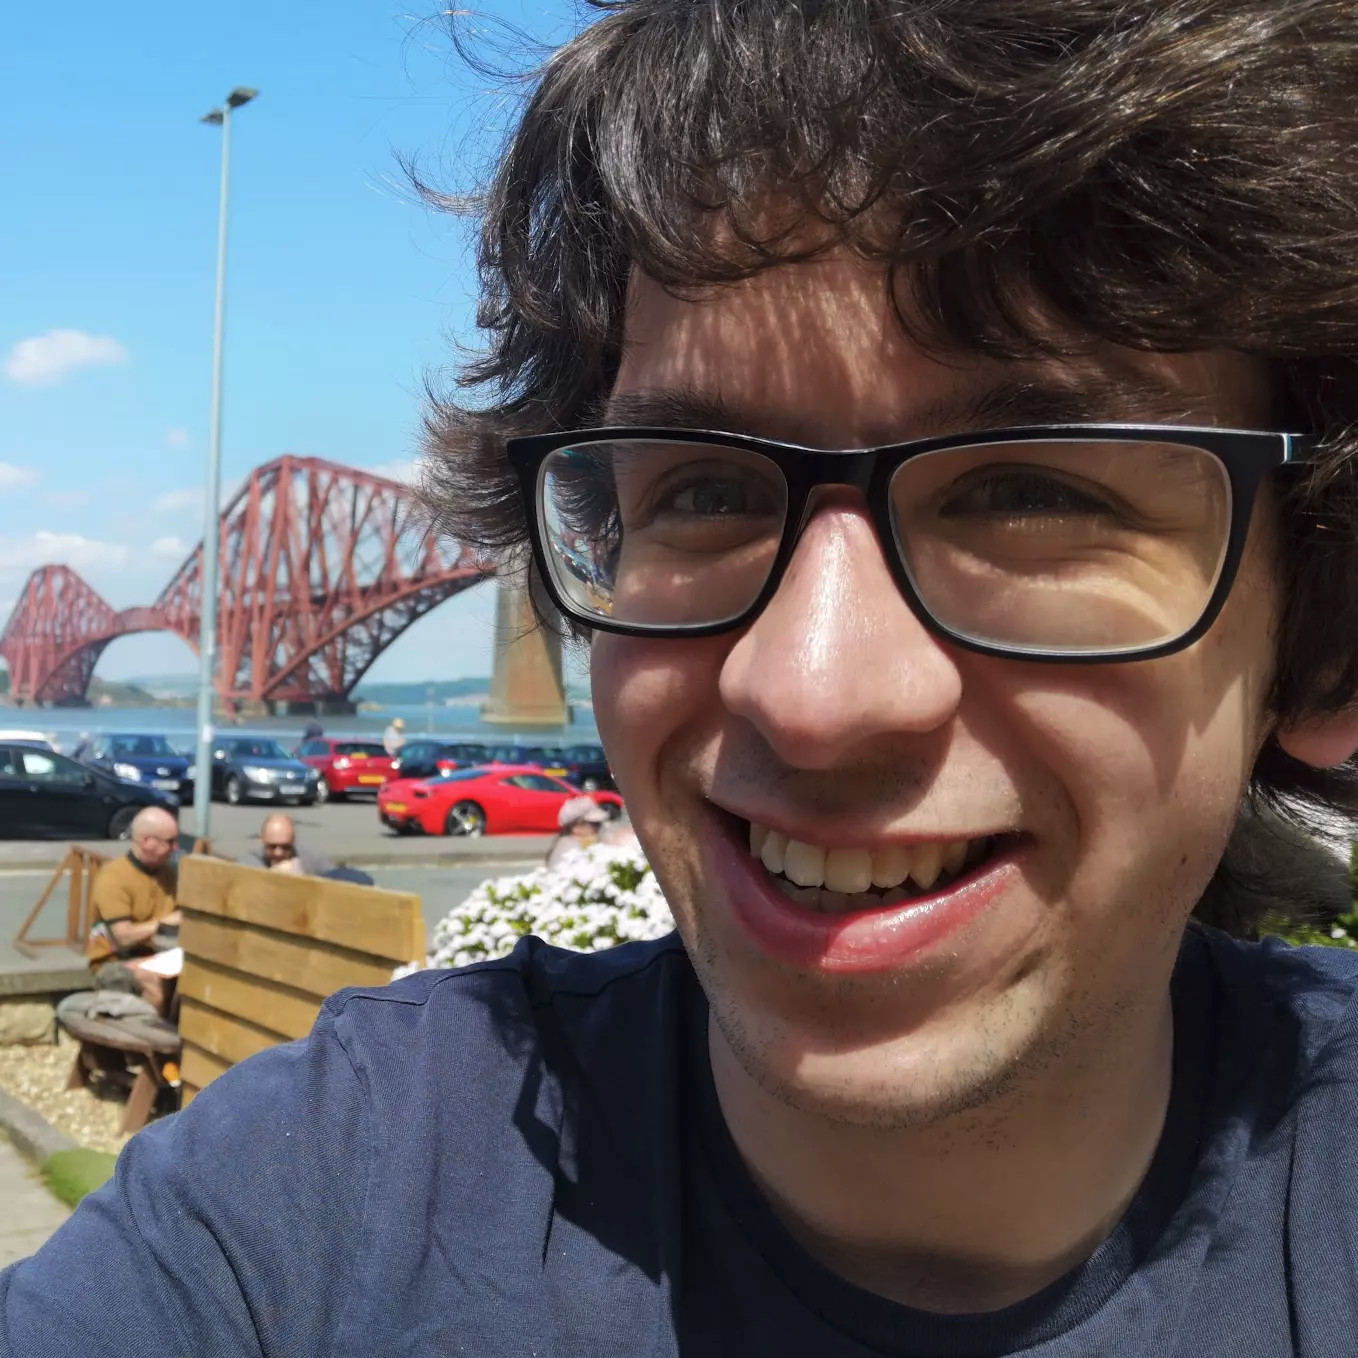
\includegraphics[width=0.2\textwidth]{imgs/me}
    }
    \qquad
    \begin{minipage}{0.7\textwidth}
        \emph{`Hi Ohad, want to do a seminar at Birmingham?'}
    \end{minipage}

    \wait
    \LARGE
    \textbf{Six months later...}
    \normalsize
    \wait

    \begin{minipage}{0.6\textwidth}
        \emph{`How about you do a seminar at Edinburgh first?'}
    \end{minipage}
    \qquad
    \raisebox{-3em}{
        
\includegraphics[width=0.2\textwidth]{imgs/ohad}
    }
\end{frame}

\begin{frame}
    \frametitle{What are we going to be talking about?}

    \centering
    \LARGE
    Digital circuits!

    \begin{center}
        \visible<2>{
            \only<-2>{
                
\includegraphics[width=0.6\textwidth]{imgs/circuit}
            }
        }
        \only<3>{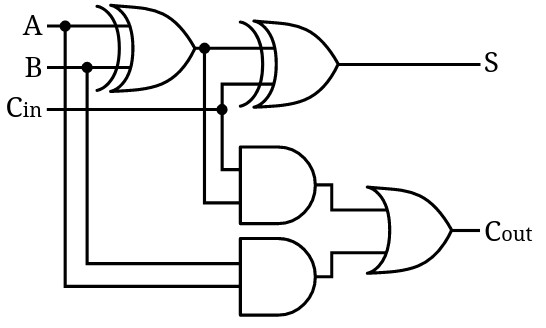
\includegraphics[width=0.6\textwidth]{imgs/adder}}
    \end{center}

\end{frame}

\begin{frame}
    \frametitle{What are we going to be talking about?}

    \centering
    \LARGE
    We want a \alert{compositional} theory of digital circuits.

    \vspace{0.5em}

    \wait
    \dsptikzfig{strings/category/f-2-2}[F][seq]
    \dsptikzfig{strings/category/f-2-2}[G][seq]

    \vspace{0.5em}

    \wait
    \dsptikzfig{strings/category/composition-2-2}[F][G][seq]
    \wait
    \quad
    \dsptikzfig{strings/monoidal/tensor-2-2}[F][G][seq]
    \wait
    \quad
    \dsptikzfig{strings/traced/trace-rhs}[F][seq]

    \wait
    \vspace{0.5em}

    \normalsize
    These operations may look familiar to you!

    \wait

    Previous attempts foiled by \alert{non-delay-guarded feedback}.

\end{frame}

\begin{frame}
    \frametitle{Joint work with...}

    \begin{minipage}{0.49\textwidth}
        \centering
        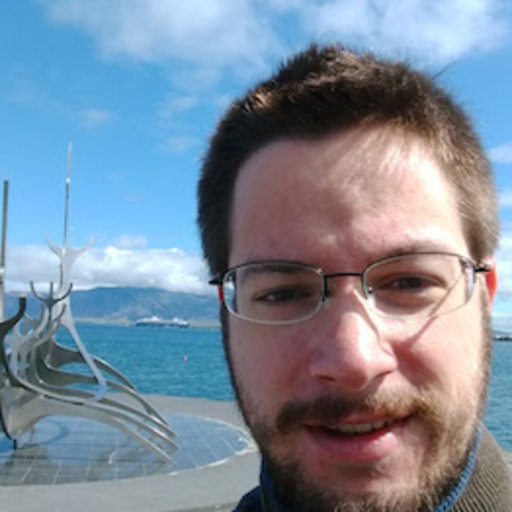
\includegraphics[width=0.5\textwidth]{imgs/sprunger}

        David Sprunger

        \scriptsize
        Indiana State University
    \end{minipage}
    \wait
    \begin{minipage}{0.49\textwidth}
        \centering
        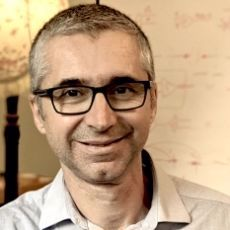
\includegraphics[width=0.5\textwidth]{imgs/ghica}

        Dan Ghica

        \scriptsize
        University of Birmingham
    \end{minipage}
\end{frame}